\documentclass{beamer}
\usepackage[utf8]{inputenc}
\usepackage[slovak]{babel}
\setbeamertemplate{navigation symbols}{}
\setbeamertemplate{footline}[frame number]

% only for this example, otherwise in .bib file
\usepackage[style=verbose,backend=biber]{biblatex}
\addbibresource{bibl.bib}

\title{Systém na podporu vypracovania bezpečnostných projektov pre malé ISVS}

\author{
    {Anton Kica} \\
    {\and} \\
    {\textit{Školiteľ}} \\
    {RNDr. Daniel Olejár, PhD}
}

\institute{FMFI Matfyz}
\date{2023}

\begin{document}

\frame{\titlepage}

\begin{frame}
    \frametitle{Žijeme v spoločnosti}
    \begin{itemize}
        \item kde postupne nastáva informatizácia v digitálnej forme
        \item štátne inštitúcie, banky, firmy využívajú d-IKT(digitálne informačné a komunikačné technológie)
        \item je potreba ochrany týchto technológií a informácií
    \end{itemize}
\end{frame}

\begin{frame}
    \frametitle{Právny podklad}
    \begin{itemize}
        \item Vyhláška č. 179/2020 Z. z. \\
            Vyhláška Úradu podpredsedu vlády Slovenskej republiky pre investície a informatizáciu, ktorou sa ustanovuje spôsob kategorizácie a obsah bezpečnostných opatrení informačných technológií verejnej správy 
            \begin{itemize}
                \item vymedzuje kategorie a obsah bezpečnostných opatrení ITVS
            \end{itemize}
        \item Zákon č. 95/2019 Z. z. \\
            Zákon o informačných technológiách vo verejnej správe a o zmene a doplnení niektorých zákonov
            \begin{itemize}
                \item vymedzuje organizáciu správy ITVS
                \item vymedzuje základné požiadavky kladené na ITVS
            \end{itemize}
    \end{itemize}
\end{frame}
\begin{frame}
    \frametitle{Menšie okno do vyhlášky č. 179/2020}
    \begin{figure}
        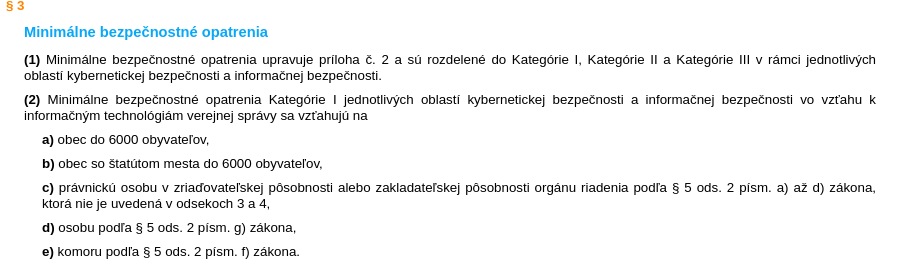
\includegraphics[width=\textwidth]{./179_2020.png}
        \caption{https://www.zakonypreludi.sk/zz/2020-179}
    \end{figure}
\end{frame}
\begin{frame}
    \frametitle{Menšie okno do vyhlášky č. 179/2020}
    MINIMÁLNE BEZPEČNOSTNÉ OPATRENIA
    \begin{itemize}
        \item A. Organizácia kybernetickej bezpečnosti a informačnej bezpečnosti \\
            Kategória I
            \begin{enumerate}[a)]
                \item Určenie pracovníka zodpovedného za koordináciu kybernetickej bezpečnosti a informačnej bezpečnosti.
                \item Vypracovanie a implementácia interného riadiaceho aktu, ktorý je pre organizáciu správcu záväzný a obsahuje najmenej
                    \begin{enumerate}[1.]
                        \item určenie povinnosti, zodpovednosti a právomoci pracovníka zodpovedného za koordináciu kybernetickej bezpečnosti a informačnej bezpečnosti,
                        \item základné zásady a opatrenia kybernetickej bezpečnosti a informačnej bezpečnosti, ktoré organizácia správcu má zavedené a riadi sa nimi.
                    \end{enumerate}
            \end{enumerate}
        \item B. Riadenie rizík kybernetickej bezpečnosti a informačnej bezpečnosti
        \item C. Personálna bezpečnosť
        \item ...
        \item P. Audit a kontrolné činnost
    \end{itemize}
\end{frame}


\begin{frame}
    \frametitle{Kde nastáva problém}
    \begin{itemize}
        \item mnoho systémov, ktoré potrebujú komunikovať s ITVS
        \item nedostatok odborníkov na KIB (kybernetickú a informačnú bezpečnosť)
        \item vrámci organizácie osoba poverená KIB nemusí mať primeranú úroveň vedomostí
    \end{itemize}
\end{frame}
\begin{frame}
    \frametitle{Cieľ našej práce}
    Predpokladáme, že vrámci organizácie manažér KIB
    \begin{itemize}
        \item nemá vedomosti z KIB
        \item nemá dostatok prostriedkov
    \end{itemize}
    my tejto osobe chceme pomôcť
    \begin{itemize}
        \item splniť si základné zákonné povinnosti
        \item zaviesť v organizácií systém ISMS
        \item udržiavať KIB na primeranej úrovni
    \end{itemize}
\end{frame}
\begin{frame}
    \frametitle{Čo nám pomôže pri tvorbe takéhoto systému}
    pár nemeckých štandardov
    \begin{itemize}
        \item BSI-Standard 200-1
        \item BSI-Standard 200-2
        \item BSI-Standard 200-3
        \item IT-Grundschutz Compendium
    \end{itemize}
\end{frame}
\begin{frame}
        
\includegraphics[width=\textwidth,height=\textheight,keepaspectratio]{./germans.png}
\end{frame}
\begin{frame}
    \frametitle{Chceme teda}
    poskytnúť systém na zavedenie ISMS, ktorý bude obsahovať interaktívny návod a
    \begin{itemize}
        \item stručne zdôvodní zákonné povinnosti
        \item poskytne referencie na detailnejšie materiály
        \item postupne bude tvoriť databázu a zbierať informácie pre KIB
    \end{itemize}
    pričom získané informácie bude možno použiť na
    \begin{itemize}
        \item analýzu rizík
        \item evidenciu bezpečnostných incidentov
        \item monitorovanie aktuálneho stavu KIB v organizácií
    \end{itemize}
    a to by mal predstavovať náš systém na podporu vypracovania bezpečnostných projektov pre malé ISVS \\ \\
\end{frame}
\begin{frame}
    \frametitle{Koniec}
    Ďakujem za vašu pozornosť
\end{frame}
\begin{frame}
    \frametitle{Pár pojmov}
    \begin{itemize}
        \item aktívum (asset)
            čokoľvek, čo má pre organizáciu hodnotu, čokoľvek, čo je:
            \begin{itemize}
                \item hmotné (zariadenia, personál..) alebo nehmotné (peniaze, informácia),
                \item môže sa stať objektom útoku a
                \item vyžaduje si ochranu
            \end{itemize}
        \item informačná bezpečnosť - 
            multiodborová disciplína, ktorá sa zaoberá
            \begin{itemize}
                \item hrozbami voči systémom/aktívam a
                \item metódami, ako aktíva pred hrozbami chrániť
            \end{itemize}
        \item kybernetický priestor -
            globálny dynamický otvorený systém, ktorý tvoria:
            \begin{itemize}
                \item telekomunikačné a počítačové siete,
                \item informačné a komunikačné systémy, ich programové vybavenie 
                \item a údaje, ktoré sa pomocou nich spracovávajú
            \end{itemize}
    \end{itemize}
    zdroj: Olejár D., Krátky úvod do informačnej a kybernetickej bezpečnosti a Malý výkladový slovník
\end{frame}
\end{document}
